

Note que como $(n_1 - 1) \cdot \frac{S_1^2}{\sigma^2} \sim \chi^2_{n_1 - 1}$ e $(n_2 - 1) \cdot \frac{S_2^2}{\sigma^2} \sim \chi^2_{n_2 - 1}$, então

\begin{equation}
(n_1 + n_2 - 2) \cdot \frac{S_p^2}{\sigma^2} \sim \chi^2_{n_1 + n_2 - 2}
\end{equation}

Daí note que

\begin{equation}
U = \frac{\overline{X}_1 - \overline{X}_2 - (\mu_1 - \mu_2)}{S_p \sqrt{\frac{1}{n_1} + \frac{1}{n_2}}} 
= \frac{\overline{X}_1 - \overline{X}_2 - (\mu_1 - \mu_2)}{\sigma \sqrt{\frac{1}{n_1} + \frac{1}{n_2}}} \cdot \sqrt{\frac{n_1 + n_2 - 2}{n_1 + n_2 - 2} \cdot \frac{S_p^2}{\sigma^2}} \sim t_{n_1 + n_2 - 2}
\end{equation}

Para $\nu = n_1 + n_2 - 2$ e $t_{\nu, \alpha/2}$ tal que

\begin{equation}
P(U > t_{\nu, \alpha/2}) = \frac{\alpha}{2}
\end{equation}

\begin{center}
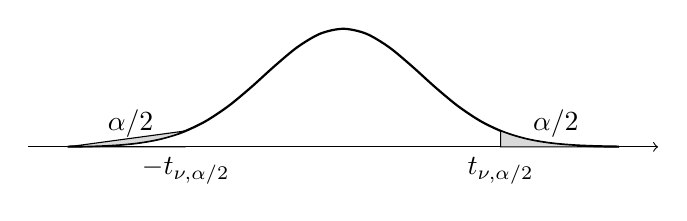
\begin{tikzpicture}
\draw[->] (-4,0) -- (4,0);
\draw[thick, domain=-3.5:3.5, smooth, variable=\x] plot ({\x}, {1.5*exp(-\x*\x/2)});
\draw[fill=gray!30] (2,0) -- plot[domain=2:3.5] ({\x}, {1.5*exp(-\x*\x/2)}) -- (3.5,0) -- cycle;
\draw[fill=gray!30] (-2,0) -- plot[domain=-3.5:-2] ({\x}, {1.5*exp(-\x*\x/2)}) -- (-3.5,0) -- cycle;
\node at (2.7,0.3) {$\alpha/2$};
\node at (-2.7,0.3) {$\alpha/2$};
\node at (2,-0.3) {$t_{\nu, \alpha/2}$};
\node at (-2,-0.3) {$-t_{\nu, \alpha/2}$};
\end{tikzpicture}
\end{center}

\begin{equation}
P\{-t_{\nu, \alpha/2} < U < t_{\nu, \alpha/2}\} = 1 - \alpha
\end{equation}

\begin{equation}
P\left\{-t_{\nu, \alpha/2} < \frac{\overline{X}_1 - \overline{X}_2 - (\mu_1 - \mu_2)}{S_p \sqrt{\frac{1}{n_1} + \frac{1}{n_2}}} < t_{\nu, \alpha/2}\right\} = 1 - \alpha
\end{equation}

\begin{equation}
\therefore P\left\{\overline{X}_1 - \overline{X}_2 - t_{\nu, \alpha/2} \cdot S_p \sqrt{\frac{1}{n_1} + \frac{1}{n_2}} < \mu_1 - \mu_2 < \overline{X}_1 - \overline{X}_2 + t_{\nu, \alpha/2} \cdot S_p \sqrt{\frac{1}{n_1} + \frac{1}{n_2}}\right\} = 1 - \alpha
\end{equation}

Isto é

\begin{equation}
IC_{1-\alpha}(\mu_1 - \mu_2) = \left[ \overline{X}_1 - \overline{X}_2 \pm t_{\nu, \alpha/2} \cdot S_p \sqrt{\frac{1}{n_1} + \frac{1}{n_2}} \right]
\end{equation}

